\section{Aufbau und Durchführung}
\label{sec:Durchführung}
\subsection{Aufbau}
Als Apparatur dient eine optische Bank, auf dieser werden ein Gegenstand "Perl L", eine Linse und ein Schirm
positioniert. Als Lichtquelle dient eine Halogenlampe.
\subsection{Verifizierung vom Abbildungsgesetz und der Linsengleichung}
In diesem Versuch wird gefordert das Abbildungsgesetz und die Linsengleichung zu verifizieren.
Zu diesem Zwecke wird eine zunächst feste Gegenstandsweite eingestellt und der Schirm entsprechend
positioniert, bis ein Scharfes Bild entsteht. Gegenstandsweite $g$, Bildweite $b$ und Bildgröße $B$ werden
aufgenommen. Für neun weitere Gegenstandsweiten werden die entsprechenden anderen Größen aufgenommen.
Diese Messung wird mit einer weiteren Sammellinse wiederholt.
\subsection{Methode nach Bessel}
Die nächste Messung verläuft nach der Methode von Bessel. Hierzu werden Gegenstand und Schirm
in einem festen Abstand $e$ aufgestellt und die Sammellinse vom Gegenstand aus verschoben bis ein scharfes Bild
auf dem Schirm entsteht. Die Bildweite $b_\mathrm{1}$ und die Gegenstandsweite $g_\mathrm{1}$ werden
notiert. Anschließend wird die Linse weiter verschoben bis erneut ein scharfes Bild erscheint.
Das Wertepaar $b_\mathrm{2}$ und $g_\mathrm{2}$ wird aufgeschrieben. Diesse Messung wird für neun
weitere Abstände $e$ durchgeführt.
Diese Methode wird auch genutzt um die chromatische Abberation zu untersuchen. Dazu wird die Messung
für funf verschiedene Abstände $e$ für blaues und rotes Licht, realisiert durch Filter, durchgeführt.
Der schematische Aufbau für diese Versuchsanordnung findet sich in Abbildung \ref{fig:bessel} wieder.
\begin{figure}
 \centering
 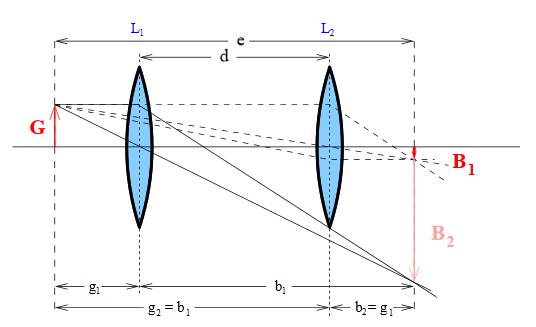
\includegraphics[width=0.5\textwidth]{bessel.png}
 \caption{Schematischer Aufbau der Apparatur nach Bessel\cite{sample}.}
 \label{fig:bessel}
 \end{figure}
\subsection{Methode von Abbe}
Für diese Messung wird ein Linsensystem aus Zerstreuungslinse und Sammellinse, in dieser Reihenfolge
vom Schirm aus gesehen, genutzt. Die beiden Linsen behalten während der Messung einen konstanten Abstand
bei und werden verschoben bis auf dem Schirm ein scharfes Bild entsteht. Die Bildweite und Gegenstandsweite
werden, bezogen auf einen Referenzpunkt hier die Mittelebene der Sammelebene, gemessen. Die
Bildgröße $B$ wird auch aufgenommen. Die Messung wird neun weitere Male wiederholt, dabei werden Linsensystem und
Schirm immer verschoben bis ein scharfes Bild entsteht.
Der schematische Aufbau für diese Versuchsanordnung findet sich in Abbildung \ref{fig:Abbe} wieder.
\begin{figure}
 \centering
 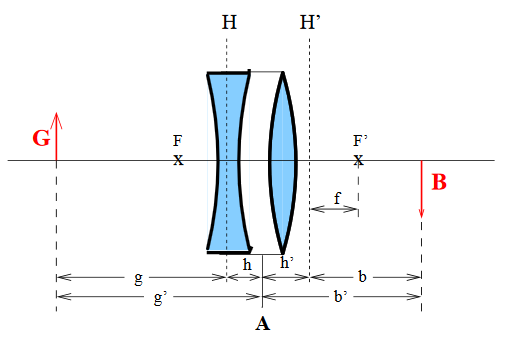
\includegraphics[width=0.5\textwidth]{abbe.png}
 \caption{Schematischer Aufbau der Apparatur nach Abbe\cite{sample}.}
 \label{fig:Abbe}
 \end{figure}
